\documentclass[
  bibliography=totoc,     % Literatur im Inhaltsverzeichnis
  captions=tableheading,  % Tabellenüberschriften
  titlepage=firstiscover, % Titelseite ist Deckblatt
]{scrartcl}

% Paket float verbessern
\usepackage{scrhack}

% Warnung, falls nochmal kompiliert werden muss
\usepackage[aux]{rerunfilecheck}

% unverzichtbare Mathe-Befehle
\usepackage{amsmath}
% viele Mathe-Symbole
\usepackage{amssymb}
% Erweiterungen für amsmath
\usepackage{mathtools}

% Fonteinstellungen
\usepackage{fontspec}
% Latin Modern Fonts werden automatisch geladen
% Alternativ zum Beispiel:
%\setromanfont{Libertinus Serif}
%\setsansfont{Libertinus Sans}
%\setmonofont{Libertinus Mono}

% Wenn man andere Schriftarten gesetzt hat,
% sollte man das Seiten-Layout neu berechnen lassen
\recalctypearea{}

% deutsche Spracheinstellungen
\usepackage[ngerman]{babel}


\usepackage[
  math-style=ISO,    % ┐
  bold-style=ISO,    % │
  sans-style=italic, % │ ISO-Standard folgen
  nabla=upright,     % │
  partial=upright,   % │
  mathrm=sym,        % ┘
  warnings-off={           % ┐
    mathtools-colon,       % │ unnötige Warnungen ausschalten
    mathtools-overbracket, % │
  },                       % ┘
]{unicode-math}

% traditionelle Fonts für Mathematik
\setmathfont{Latin Modern Math}
% Alternativ zum Beispiel:
%\setmathfont{Libertinus Math}

\setmathfont{XITS Math}[range={scr, bfscr}]
\setmathfont{XITS Math}[range={cal, bfcal}, StylisticSet=1]

% Zahlen und Einheiten
\usepackage[
  locale=DE,                   % deutsche Einstellungen
  separate-uncertainty=true,   % immer Unsicherheit mit \pm
  per-mode=symbol-or-fraction, % / in inline math, fraction in display math
]{siunitx}

% chemische Formeln
\usepackage[
  version=4,
  math-greek=default, % ┐ mit unicode-math zusammenarbeiten
  text-greek=default, % ┘
]{mhchem}

% richtige Anführungszeichen
\usepackage[autostyle]{csquotes}

% schöne Brüche im Text
\usepackage{xfrac}

% Standardplatzierung für Floats einstellen
\usepackage{float}
\floatplacement{figure}{htbp}
\floatplacement{table}{htbp}

% Floats innerhalb einer Section halten
\usepackage[
  section, % Floats innerhalb der Section halten
  below,   % unterhalb der Section aber auf der selben Seite ist ok
]{placeins}

% Seite drehen für breite Tabellen: landscape Umgebung
\usepackage{pdflscape}

% Captions schöner machen.
\usepackage[
  labelfont=bf,        % Tabelle x: Abbildung y: ist jetzt fett
  font=small,          % Schrift etwas kleiner als Dokument
  width=0.9\textwidth, % maximale Breite einer Caption schmaler
]{caption}
% subfigure, subtable, subref
\usepackage{subcaption}

% Grafiken können eingebunden werden
\usepackage{graphicx}

% schöne Tabellen
\usepackage{tabularray}
\UseTblrLibrary{booktabs, siunitx}

% Verbesserungen am Schriftbild
\usepackage{microtype}

% Literaturverzeichnis
\usepackage[
  backend=biber,
]{biblatex}
% Quellendatenbank
\addbibresource{lit.bib}
\addbibresource{programme.bib}

% Hyperlinks im Dokument
\usepackage[
  german,
  unicode,        % Unicode in PDF-Attributen erlauben
  pdfusetitle,    % Titel, Autoren und Datum als PDF-Attribute
  pdfcreator={},  % ┐ PDF-Attribute säubern
  pdfproducer={}, % ┘
]{hyperref}
% erweiterte Bookmarks im PDF
\usepackage{bookmark}

% Trennung von Wörtern mit Strichen
\usepackage[shortcuts]{extdash}

\author{%
  Vincent Wirsdörfer\\%
  \href{mailto:vincent.wirsdoerfer@udo.edu}{authorA@udo.edu}%
  \and%
  Joris Daus\\%
  \href{mailto:joris.daus@udo.edu}{authorB@udo.edu}%
}
\publishers{TU Dortmund – Fakultät Physik}


\begin{document}
\section{Zielsetzung}
\label{sec:Theorie}

In folgendem Versuch wird die Erzeugung freier Elektronen durch thermische Energie untersucht. Diese sollen durch den 
glühelektrischen Effekt freigesetzt werden. Dies geschieht mithilfe einer Hochvakuumdiode. Für ein besseres Verständnis 
der Erzeugung von freien Elektronen soll außerdem die Funktionsweise der Hochvakuumdiode untersucht werden. 

\section{Theorie}

Wie auch bei dem Versuch zum Photoeffekt werden hier die freien Elektronen aus einem Metall gelöst. Hierbei ist es 
wichtig, dass es sich um ein Metall handelt, da Metalle besondere physikalische Eigenschaften haben, auf die im 
Folgenden genauer eingegangen wird. Metalle sind meist kristalline Festkörper. Das bedeutet, dass die Atome, aus denen 
das Metall besteht in einer Gitterstruktur angeordnet sind. Dabei sind praktisch alle Atome ionisiert. Dies hat zur Folge, 
dass es freie Leitungselektronen gibt. Nun hat diese Aufteilung der positiven und negativen Ladungen zur Folge, dass sich 
im Metallinneren in nullter Näherung ein konstantes positives Potential einstellt. So entsteht zur Außenwelt eine 
Potentialbarriere, für welche die Elektronen Energie benötigen, um diese zu Überwinden. Dies kann auch als folgender 
Potentialtopf aufgeefasst werden.

\begin{figure}
    \centering
    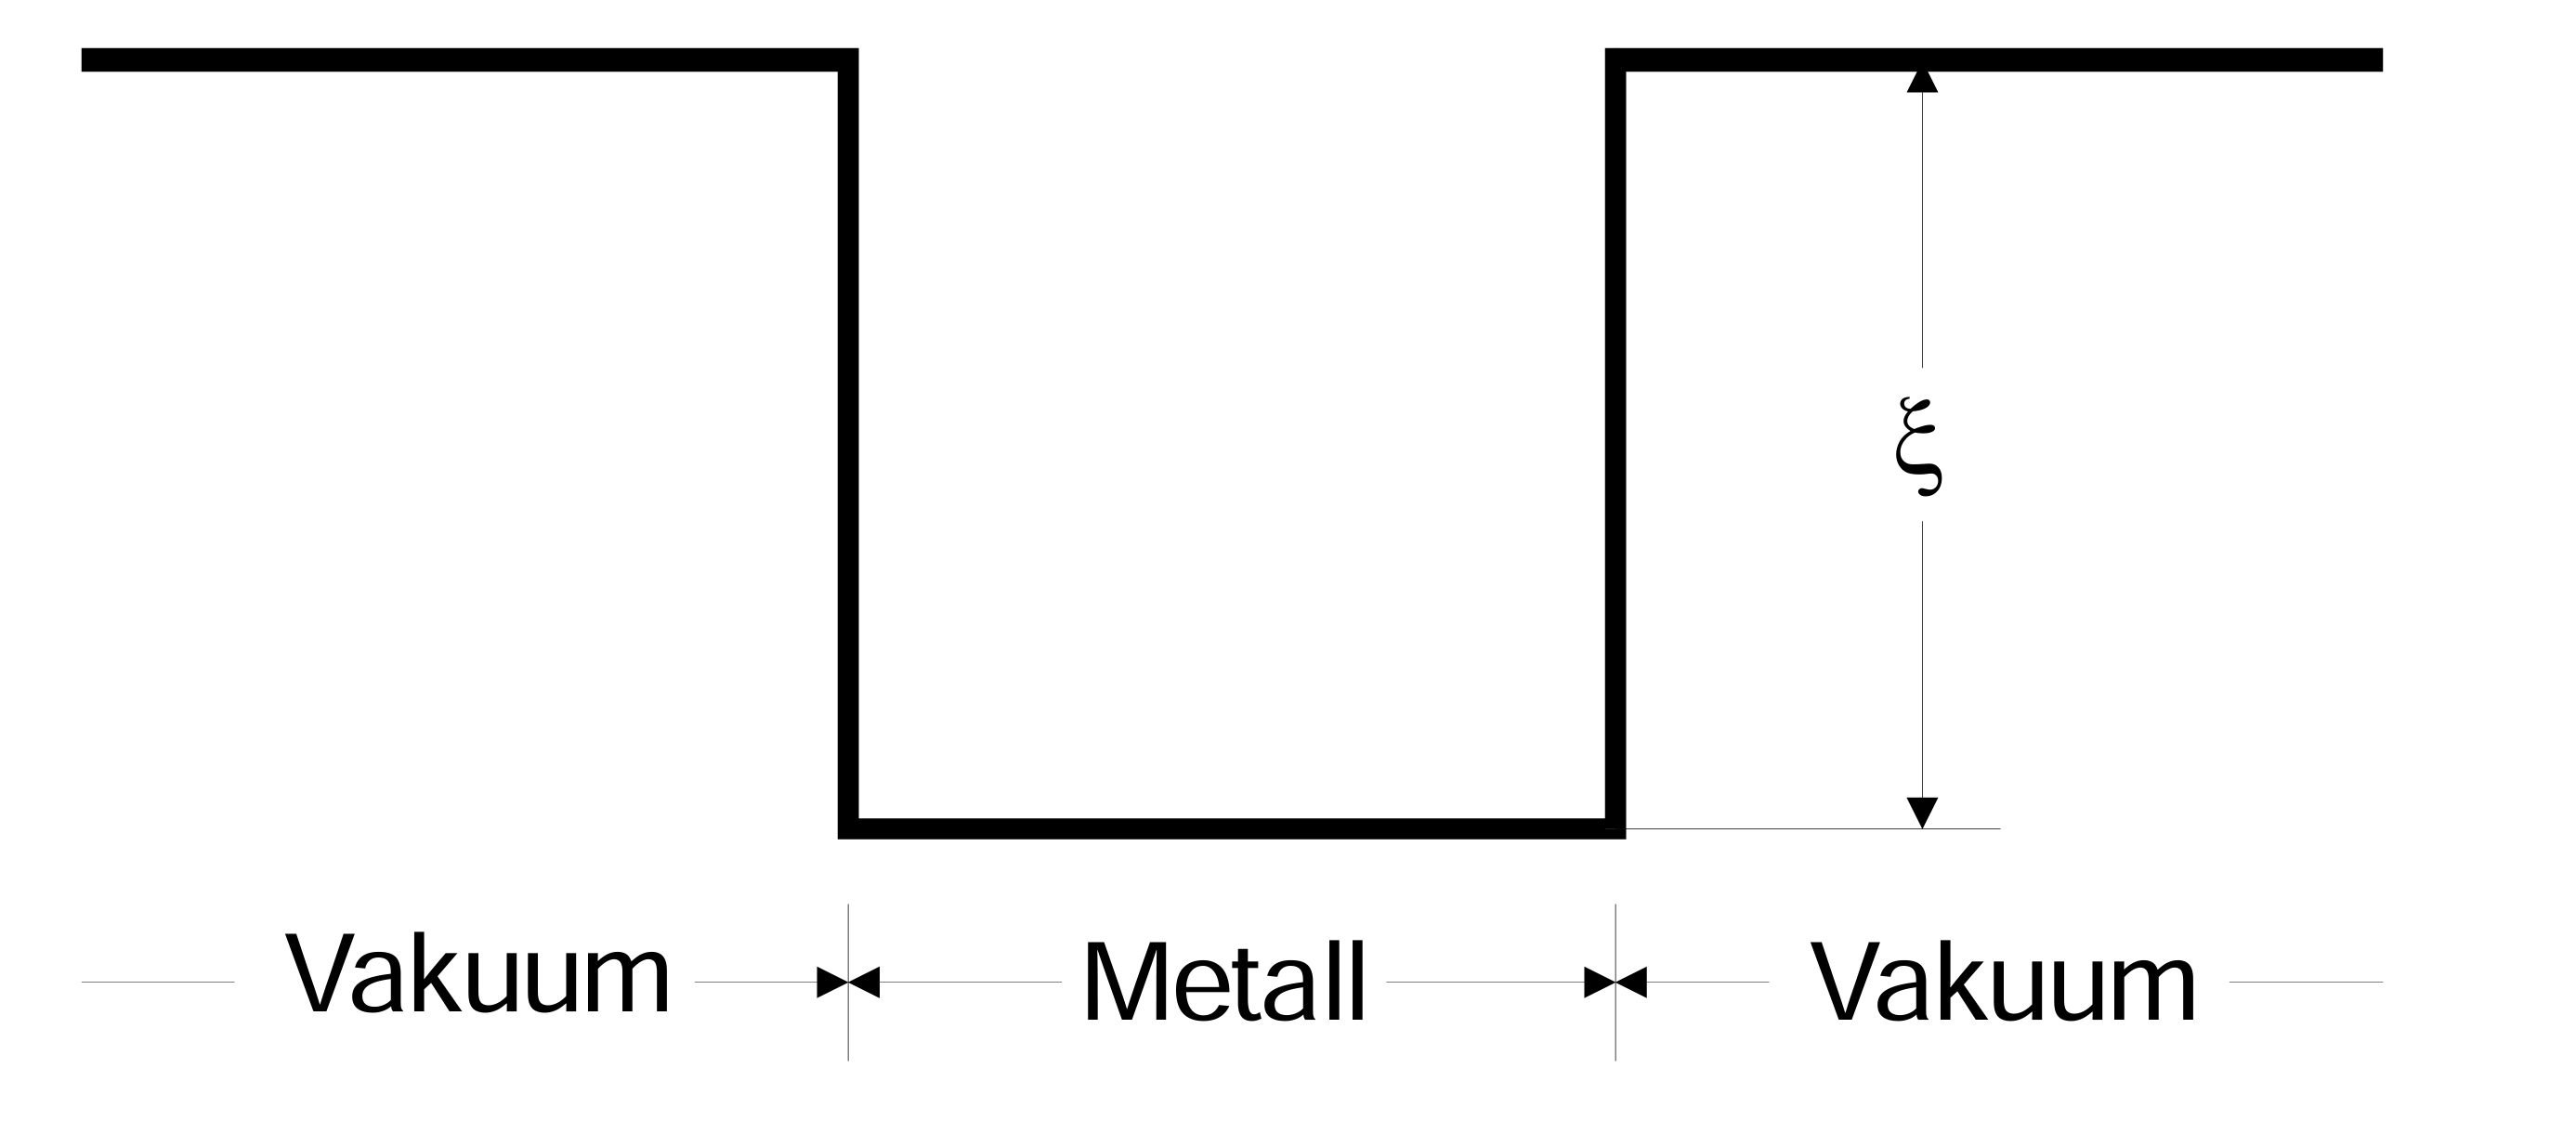
\includegraphics[width=0.69\textwidth]{Potentialtopf.png}
    \caption{Darstellung der Energiehürde für Elektronen.}
\end{figure}

\noindent Die Wahrscheinlichkeit ein Elektron Abhängig von seiner Energie anzutreffen, ist durch die Fermi-Diracsche 
Verteilungsfunktion 

\begin{equation}
    f(E)=\frac{1}{\exp{(\frac{E-\zeta}{k_B T})} + 1}
    \label{eqn:Fermi-Dirac}
\end{equation}

\noindent gegeben. Dabei ist $\zeta$ Die Fermische Grenzenergie. Bei Zimmertemperatur ist diese für alle Metalle 
$\zeta >>k_B T$, weshalb halb \autoref{eqn:Fermi-Dirac} sich zu 

\begin{equation*}
    f(E) \approx \exp{(\frac{\zeta - E}{k_B T})}
\end{equation*}

\noindent vereinfacht.


\subsection{Hochvakuumdiode}
Die Messung der freien Elektronen geschieht durch eine Hochvakuumdiode. Dabei herrscht, wie der Name schon vermuten 
lässt, ein Vakuum im Inneren der Diode. Die Diode besteht aus einer Kathode und einer Anode. An der Kathode sollen 
die freien Elektronen entstehen und dann zur Anode gelangen. An der Kathode und der Anode liegt eine Spannung an, 
welche Saugspannung genannt wird. Sie sorgt dafür dass die freien Elektronen sich gezielt Richtung Anode bewegen. 
Da ein Vakuum herrscht fließt kein Strom, wenn keine freien Elektronen vorhanden sind. Dies ist im Vakuum der Fall. 
Wird nun die Heizspannung eingeschaltet, um freie Elektronen zu erzeugen, so gehen Elektronen von der Kathode zur 
Anode und es fließt (per Definition) ein Strom. Dieser Strom ändert sich je nach Saugspannung. Diese Abhängigkeit 
wird durch die Kennlinie der Hochvakuumdiode verdeutlicht. 

\begin{figure}
    \centering
    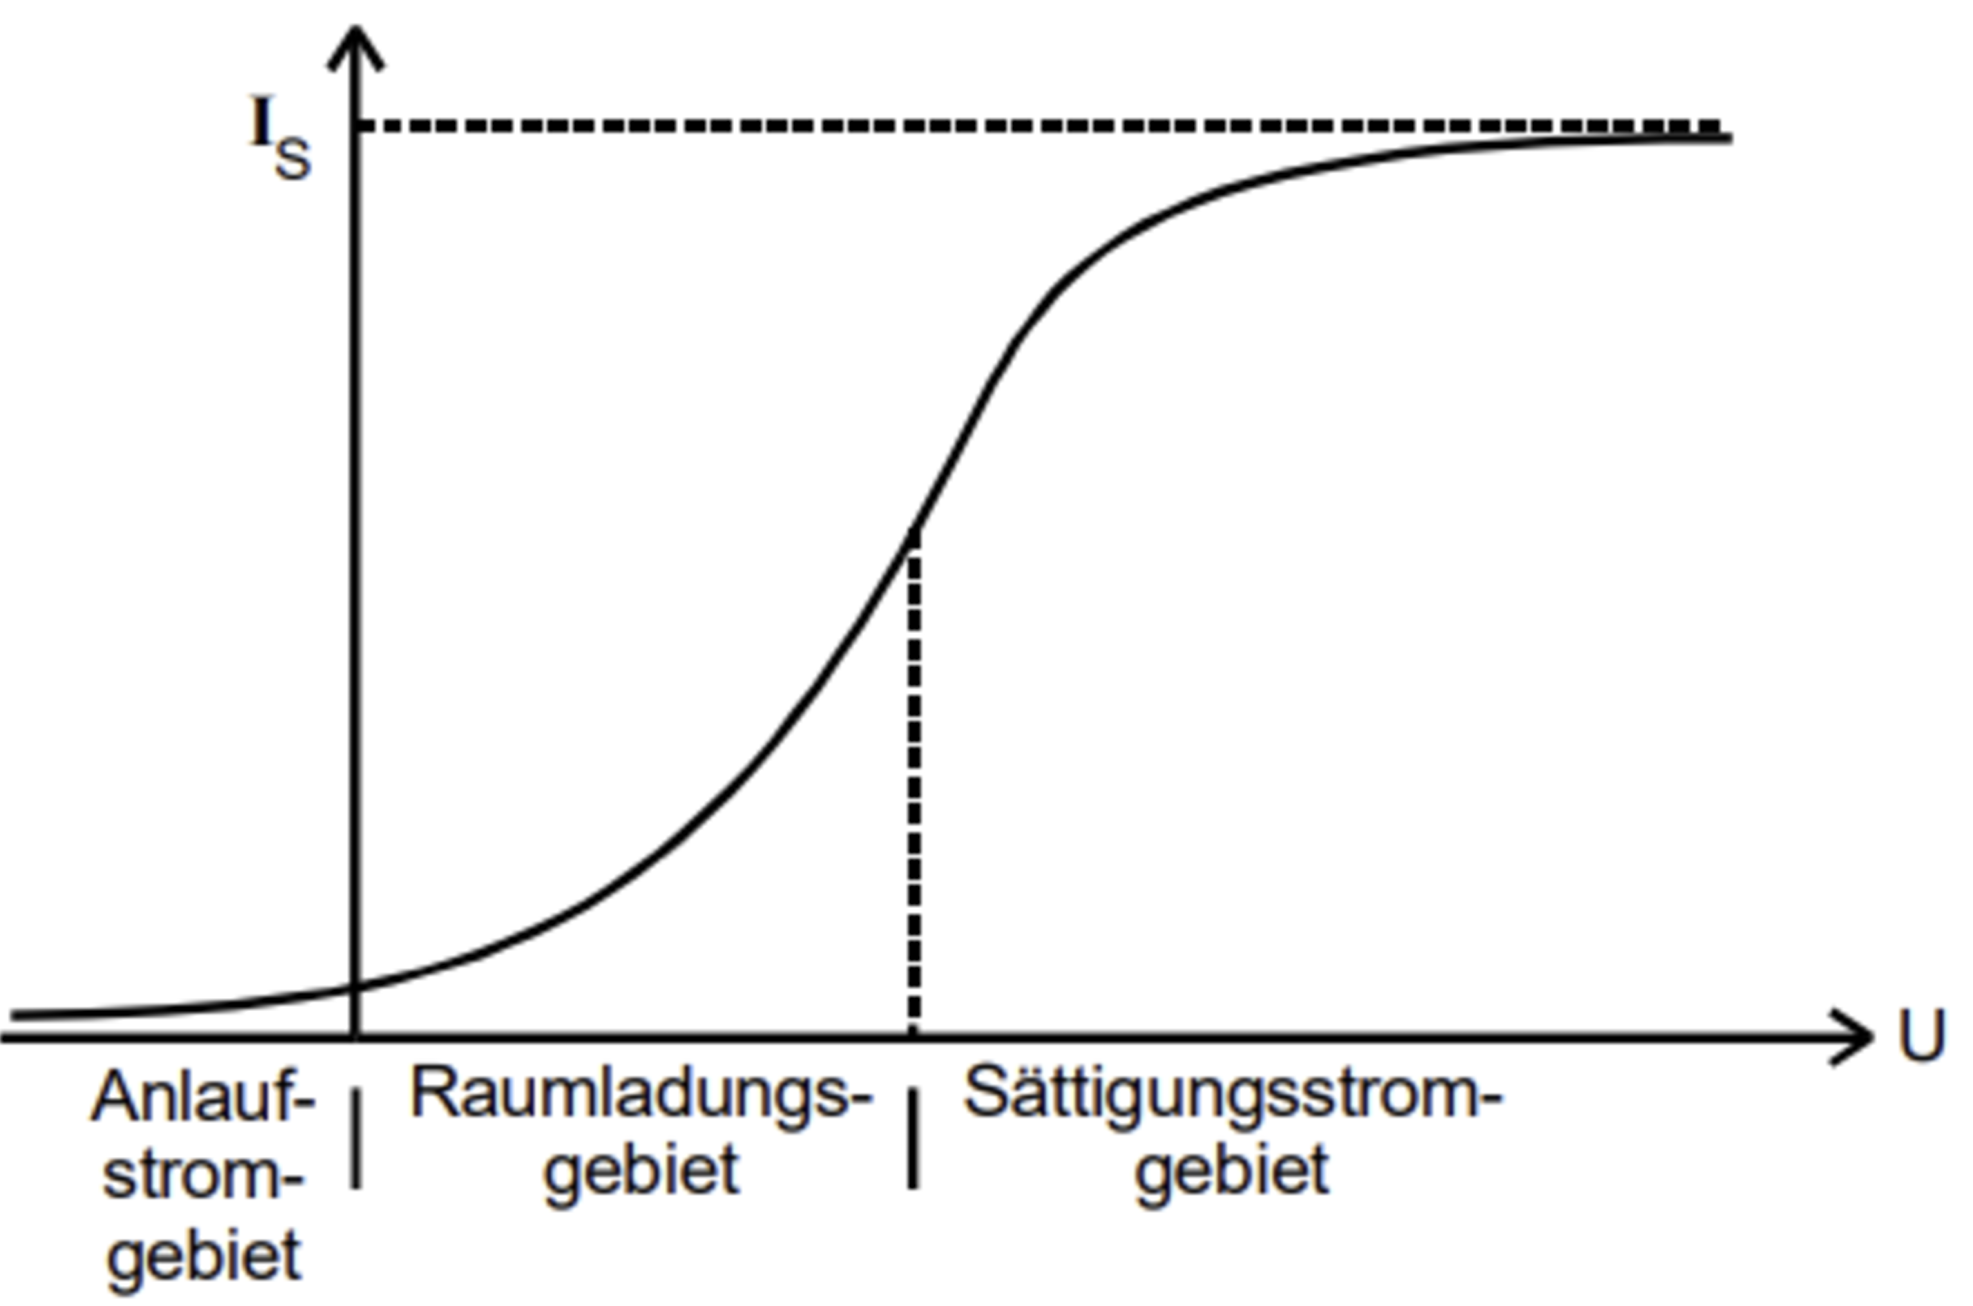
\includegraphics[width=0.9\textwidth]{Kennlinie.png}
    \caption{Kennlinie der Hochvakuumdiode.}
\end{figure}

\noindent Die Kennlinie wird in drei Bereiche unterteilt: Das Anlaufstromstromgebiet, Raumladungsgebiet und 
Sättigungsgebiet.\\

\noindent Das Anlaufstromgebiet geht bis zu einer Spannung von \qty{0}{\volt}. Theoretisch sollte kein Strom 
fließen, da Elektronen nicht aufgrund von Hitze aus dem Metall austreten und keine Saugspannung anliegt. 
Dies ist jedoch nicht der Fall, da Elektronen nie keine Energie besitzen. Sie besitzen außerdem auch immer 
eine Geschwindigkeit. Es kann also passieren, dass Elektronen sich spontan vom Metall lösen und ihre 
Eigengeschwindigkeit ausreicht, um die Strecke zur Anode zu überwinden. Dieses Anlaufstromgebiet nimmt jedoch 
exponentiell mit negativer Spannung ab. So lässt sich die folgende Gesetzmäßigkeit aufstellen:

\begin{equation*}
    j(U) = j_0 \exp(-\frac{\text{e}_0 \phi_A + \text{e}_0 U}{k_B T}) = \text{const} \exp(-\frac{\text{e}_0 U}{k_B T})
\end{equation*}

\noindent $\text{e}_0 \phi_A$ ist dabei die Austrittsarbeit des Anodenmaterials. \\

\noindent Das Raumladungsgebiet ist der Zwischenbereich von Anlaufstromgebiet bis hin zum Sättigungsstromgebiet. 
Es wird durch das Langmuir-Schottkysche Raumladungsgesetz beschrieben. Dieses lautet 

\begin{equation}
    j = \frac 4 9 \varepsilon_0 \sqrt{\frac{2\text{e}_0} {\text{m}_0} } \frac{V^{\frac 3 2}}{a^2}
\end{equation}



\section{Vorbereitung}

\section{Fehlerrechnung}
\end{document}